\documentclass[a4paper, 11pt]{article}

\usepackage[left=2cm, top=3cm, text={17cm, 24cm}]{geometry}
\usepackage[czech]{babel}
\usepackage{graphicx}
\usepackage{hyperref}
\usepackage{subcaption}
\usepackage{dirtree}


\title{Dokumentace k projektu IMP \\ \Large Aplikace ovládaná pomocí rotačního enkodéru KX/Y-040}
\author{Ondřej Koumar, xkouma02}
\date{\today}

\begin{document}

\maketitle

\section{Úvod do problematiky}\label{1:uvod}
Projekt je řešený na platformě FITkit3, kde je vsazen mikrokontrolér Kinetis MK60DN512VMD10. s použitím dvou externích rotačních enkodérů typu \mbox{KX/Y-40.}
Pro interakci s uživatelem je použito sériové komunikační rozhraní UART, přesněji pouze odesílací část.
Dále, aby měl uživatel zpětnou vazbu svých akcí, každá interakce s deskou způsobí zaznění tónu na integrovaném bzučáku, délka a výška tónu je dle použitého zařízení, případně směru pohybu daným zařízením (platí pro rotační enkodéry). 

\subsection{Rotační enkodér KX/Y-040}\label{1_1:rot_enc}

Rotační enkodér má pět pinů, které se dají zapojit.
\begin{figure}[h]
    \centering
    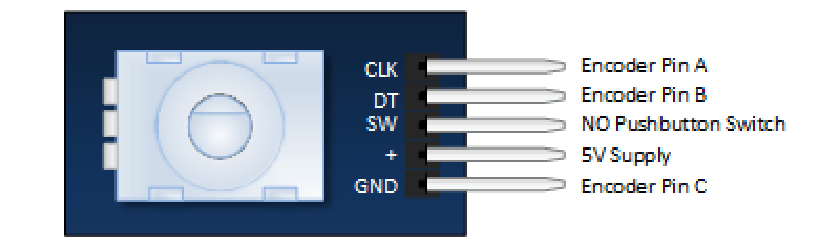
\includegraphics[width=0.8\linewidth]{images/rotary_encoder_pins.png}
    \caption{Piny rotačního enkodéru}
    \label{img:rot_enc_pins}
\end{figure}

Vždy je potřeba mít zapojenou zem a zdroj napětí (piny \emph{GND} a \emph{+}), další piny dle očekávané funkcionality.
Aby mohl uživatel na mikrokontroléru správně přečíst otočení libovolným směrem enkodéru, je potřeba zapojit piny \emph{CLK} a \emph{DT}. Pro čtení stisknutí knoflíku je potřeba zapojit pin \emph{SW}.
Výchozí hodnota na těchto pinech je log. 1.

\subsubsection{Snímání pohybu}\label{1_1_1:snimani}

Pro snímání pohybu je třeba ještě zjistit, jak rotační enkodér funguje uvnitř.
Mějme tři výstupy rotačního enkodéru zobrazeny na obrázku \ref{img:rot_enc_config}, kde výstup \emph{A} je spojen s pinem \emph{CLK}, výstup \emph{B} je spojen s pinem \emph{DT} a výstup \emph{C} vede do země.

\begin{figure}[t]
    \centering
    
    \begin{subfigure}{0.4\textwidth}
        \centering
        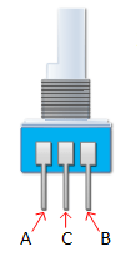
\includegraphics[]{images/rotary_encoder_outputs.png}
        \caption{Vnější konfigurace}
        \label{img:rot_enc_config}
    \end{subfigure}
    % Add some space between subfigures
    \hspace{2em}
    \begin{subfigure}{0.4\textwidth}
        \centering
        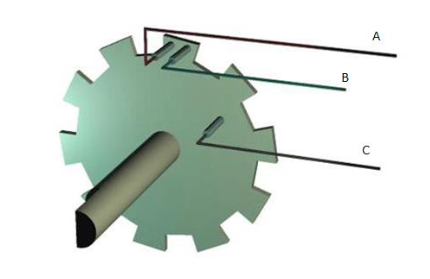
\includegraphics[width=\linewidth]{images/rotary_encoder_switches.png}
        \caption{Vnitřní spínače}
        \label{img:rot_enc_switches}
    \end{subfigure}

    \caption{Výstupy rotačního enkodéru}
    \label{img:rot_enc_outputs}
\end{figure}

Přívod napětí je přímo spojen s piny \emph{CLK} a \emph{DT} přes dva pull-up rezistory. 
Právě díky tomu je výchozí hodnota na těchto pinech log. 1.
Na obrázku \ref{img:rot_enc_switches} je vidět mechanismus spínání.
V tomto konkrétním případě jsou oba spínače otevřeny a proud jde ze zdroje napětí přímo do země.
Pokud by byly spínače zavřeny, a tedy signály \emph{A} a \emph{B} byly \uv{mimo zub} kolečka enkodéru, proud by mohl téct jedině do pinů \emph{CLK} a \emph{DT}.

Díky tomu se dá poznat, zda se rotačním enkodérem pohybuje po směru nebo proti směru hodinových ručiček.
Z obrázku lze vidět, že při pootočení knoflíku enkodéru o zhruba čtvrtinu otočky po směru hodinových ručiček se změní signál \emph{A} a výstup pinu \emph{CLK} bude log. 1, při otočení na druhou stranu se jako první změní signál \emph{B} a na výstupu pinu \emph{DT} bude log. 1. Po postupném otáčení dále se změní i signál druhý.

\subsubsection{Postupná změna signálů A a B při plném otočení}\label{1_1_2:otoceni}

Mějme stav, kde oba spínače jsou uzavřeny, tedy oba signály \uv{sedí mezi zuby}. Jako příklad vezměme pouze otočení proti směru hodinových ručiček\footnote{Po směru hodinových ručiček by sekvence vypadala stejně, jen by se prohodilo pořadí, ve kterém se hodnoty signálů mění.}.
Zpočátku bude výstup signálů \emph{CLK (A)} i \emph{DT (B)} na log. 1.

Při otočení o čtvrtinu se signál B spojí se signálem C, tedy se zemí a na výstupu \emph{DT} bude log. 0.
Po dalším kroku se zavře spínač \emph{AC}, díky čemuž je vygenerována log. 0 i na výstupu \emph{CLK}.
Dalším krokem se dostaneme do stavu, kdy spínač \emph{BC} je otevřený, \emph{AC} stále zavřený a ve finále jsou oba spínače opět otevřené a na oba výstupy se znovu generuje log. 1.

\subsection{UART (Universal Asynchronous Reciever Transmitter)}\label{1_2:uart}

UART je rozhraní pro asynchronní sériovou komunikaci mezi dvěma zařízeními.
Má konfigurovatelné parametry typu formát datového slova a přenosová rychlost.
Pro tento projekt stačí, abychom si definovali tři důležité principy.
\begin{itemize}
    \item \textbf{Baud rate}\,--\,pro dnešní počítačové systémy ekvivalent k \emph{bit rate}. Není tomu ale vždycky tak; jedná se o počet změn signálu za sekundu, kdy změna signálu může být popsána i více bity. 
    \item \textbf{Parita}\,--\,technika používaná pro kontrolu integrity dat v datovém přenosu. Může být sudá nebo lichá; posledním (paritním) bitem je datové slovo doplněno tak, aby počet jedniček ve slově byl buď sudý nebo lichý\footnote{Berme v potaz pouze jeden paritní bit.}.
    \item \textbf{Synchronizace}\,--\,je potřeba, aby generátor hodinových pulsů přijímače běžel na co \uv{nejstejnější} frekvenci jako generátor vysílače. Synchronizace se provádí předem dohodnutou změnou na datovém vodiči, v případě UARTu se jedná o přechod z log. 1 do log. 0.
\end{itemize}

\subsubsection{Komunikace mezi dvěma zařízeními}\label{1_2_1:komunikace}

Vysílač zahájí přenos datového slova tzv. \emph{start bitem}, který je právě již zmiňovanou dohodnutou změnou na datovém vodiči z klidové úrovně do opačné.
Další bit je už datový, stejně jako 7 dalších\footnote{Může být i jiný počet, obě strany se ale musí předem dohodnout.}. Za posledním vyslaným datovým, případně paritním bitem je vyslán minimálně jeden stop bit, který má vždy hodnotu klidového stavu. Ten slouží k tomu, aby byla jasně oddělena datová slova, zároveň tím ale přijímač získává dostatek času ke zpracování přijímaných dat.

\section{Implementovaná aplikace}\label{2:aplikace}

Pro implementaci byla jako aplikace vybrána jednoduchá kalkulačka ovládaná pomocí dvou rotačních enkodérů a tlačítka SW6 na desce.

\subsection{Návod na použití a uživatelské interakce}\label{2_1:navod}

Otáčením knoflíku jednoho rotačního enkodéru se vybírá první operand.
Každým otočením po směru hodinových ručiček se zvýší hodnota operandu o 1, proti směru se o 1 sníží.
Stisknutím tlačítka prvního enkodéru se výběr operandu potvrdí.

Po potvrzení se zobrazí výzva pro výběr operátoru. V základu je jich šest\,--\,výčtem sčítání, odčítání, násobení, dělení, druhá odmocnina a obecná mocnina.
Stisknutím knoflíku se zvolí operátor.
V případě výběru druhé odmocniny se rovnou spočítá výsledek, jinak se pokračuje na výběr druhého operandu, který probíhá stejně jako výběr prvního.

Po výběru druhého operandu následuje výpočet a uživateli se vypíše výsledek, případně chybová hláška, pokud uživatel zadal nedefinovanou dvojici operandů pro danou funkci.

\subsubsection{Pole předešlých výsledků}\label{2_1_1:predesle_vysledky}

Alternativně lze vybírat z pole posledních výsledků.
K tomu se uživatel dostane stisknutím knoflíku na druhém enkodéru, otáčením si pak může vybrat z 5 posledních vypočtených výsledků\footnote{V kódu lze jednoduše toto číslo změnit.}.
Opětovným stisknutím knoflíku je vybrán operand z pole předešlých výsledků.

\subsubsection{Floating-point čísla}\label{2_1_2:floating_point}

Díky operacím, jako je \texttt{sqrt()}, \texttt{pow()} nebo dělení, často se ve výsledku vyskytnou desetinná čísla. 
Kalkulačka má plnou podporu desetinných čísel, ale musí se vybrat z předešlých výsledků, protože při výběru operandů otáčením knoflíku se pouze inkrementuje nebo dekrementuje celé číslo o 1.

Výpis desetinných čísel je podporován do osmi desetinných míst.

\subsection{Implementační detaily}\label{2_2:implementace}

\subsubsection{Souborová struktura}\label{2_2_1:struktura}
Struktura zdrojových a hlavičkových souborů je na obrázku \ref{img:zdrojove_soubory}. Hlavní funkcionalita aplikace je v~souborech \emph{calculator.c}, \emph{matlib.c} a \emph{fsm.c}. V souboru \emph{result\textunderscore array.c} je pak definováno pole předešlých výsledků, se kterým se pracuje v hlavním API aplikace. \emph{uart.c} obsahuje funkce pro práci s UARTem, včetně jeho inicializace, \emph{common.c} pak definuje funkce a datové struktury společné pro celý program. V \emph{main.c} je pak hlavní smyčka programu.

\begin{figure}[t]
    \centering
    \begin{minipage}{0.26\textwidth}
        \dirtree{%
        .1 Sources/.
          .2 headers/.
            .3 calculator.h.
            .3 common.h.
            .3 fsm.h.
            .3 matlib.h.
            .3 result\textunderscore array.h.
            .3 uart.h.
          .2 calculator.c.
          .2 common.c.
          .2 fsm.c.
          .2 main.c.
          .2 matlib.c.
          .2 result\textunderscore array.c.
          .2 uart.c.
        }
    \end{minipage}
    \caption{Zdrojové a hlavičkové soubory}
    \label{img:zdrojove_soubory}
\end{figure}

\subsubsection{API}\label{2_2_2:api}

Hlavní programové API je definováno v souboru \emph{calculator.c}.
Zde se nachází například funkce \\ \texttt{PickNumber()}, \texttt{PickFromPreviousResults()}, \texttt{CalculateResult()}, \texttt{DisplayOperand()} a další pomocné funkce.
Z~pohledu hlavní programové smyčky jsou nejpodstatnější čtyři funkce:
\begin{itemize}
    \item \texttt{PickNumber()}: Přečte uživatelskou interakci s deskou\footnote{Provolává funkci \texttt{ReadBoardInteraction()}, která aktivně čeká.} a průběžně ukazuje uživateli, co má zrovna vybráno a co může potvrdit. Po potvrzení operandu zmáčknutím knoflíku funkce vrací hodnotu operandu.
    \item \texttt{PickOperator()}: Taktéž čeká na interakci s deskou, průběžně ukazuje aktuální operátor a potvrdí se stisknutím knoflíku.
    \item \texttt{CalculateResult()}: Po vybrání obou operandů a operátoru se zavolá příslušná funkce z \emph{matlib.c} a vypočte se výsledek operace, případně uloží typ chyby.
    \item \texttt{DisplayResult()}: Zobrazí uživateli do terminálu buď výsledek operace, nebo chybovou hlášku.
\end{itemize}

\subsubsection{Datové struktury}\label{2_2_3:struktury}

Hlavní datové struktury jsou definovány v \emph{common.h}. 
Struktura, která slouží pro předávání výsledků a operandů mezi funkcemi, se nazývá \texttt{CalcData}.

Je to datová struktura obsahující:
\begin{itemize}
    \item informace o datovém typu výsledku (enum \texttt{Type}),
    \item výsledek samotný\,--\,int xor float, a tedy je použita unie \texttt{Value},
    \item informace o chybě, která při výpočtu nastala, enum \texttt{FaultType}, výchozí hodnota je \texttt{NONE}.
\end{itemize}

Složitost této datové struktury je dána podporou floating-point čísel a operací s nimi. 
Je třeba mít informaci o typu výsledku, aby se dalo přistoupit do výsledkové unie.

Díky enumerátoru \texttt{FaultType} je pak možné při zobrazování výsledku uživateli místo číselného výsledku zobrazit chybovou hlášku, aniž by nás zajímala hodnota v rámci výsledkové unie.

\subsubsection{Konečný automat čtení vstupu od uživatele}\label{2_2_4:fsm}

\begin{figure}[t]
    \centering
    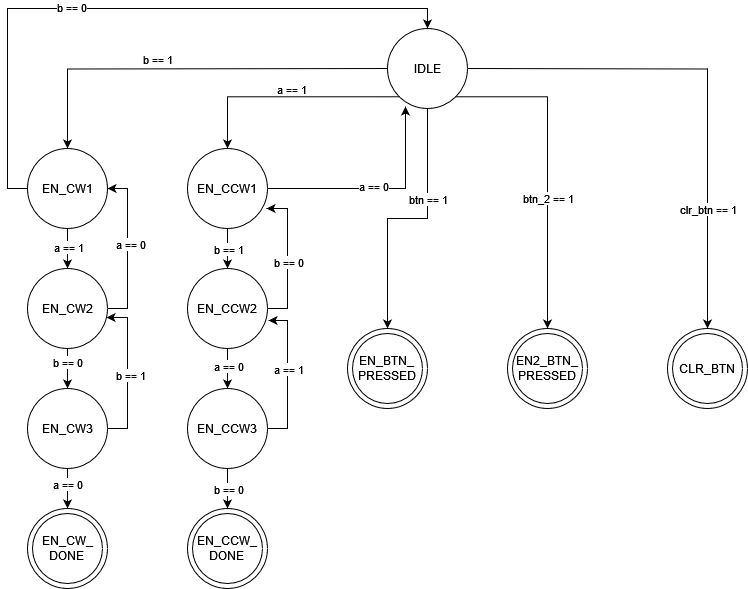
\includegraphics[width=0.8\linewidth]{images/fsm.png}
    \caption{Stavový automat čtení vstupu od uživatele}
    \label{img:fsm}
\end{figure}

Implementaci konečného automatu lze nalézt v souboru \emph{fsm.c} ve funkci \texttt{ReadBoardInteraction()}.
Tato funkce bere jeden parametr, a to \texttt{mode}, který indikuje, zda se vybírá operand inkrementací/de\-kre\-men\-ta\-cí (mód 1) celého čísla, nebo se vybírá z pole posledních výsledků (mód 2).

Konečný automat zobrazený na obrázku \ref{img:fsm} platí pouze pro mód 1. 
V případě módu 2 je automat skoro stejný, nicméně v něm chybí větev vedoucí do koncového stavu \texttt{EN2\textunderscore BTN\textunderscore PRESSED}.
Důvod je ten, že v módu 1 je možné provádět všechny operace s enkodérem 1 a stisknout knoflík enkodéru 2, zatímco v módu 2 se dá pouze interagovat s enkodérem 2 v jeho plném rozsahu.

V rámci konečného automatu jsou naimplementovány stavy \texttt{EN\textunderscore CW1}, \texttt{EN\textunderscore CW2}, \texttt{EN\textunderscore CW3}, \texttt{EN\textunderscore CW\textunderscore DONE}, stejně tak pro CCW.
Značí to postupné otáčení rotačního enkodéru po směru hodinových ručiček (CW) a proti směru hodinových ručiček (CCW), jak je popsáno v kapitole \ref{1_1_1:snimani}.
Pokud je pootočeno jedním nebo druhým směrem, pak stisknutí knoflíků, případně tlačítka na desce, není dostupné.
Ty se dají stisknout ve stavu \texttt{IDLE}, ve kterém automat zůstává, pokud není žádná aktivní interakce od uživatele.

\section{Zhodnocení}\label{3:zhodnoceni}

Implementací výše uvedených vlastností byla vytvořena jednoduchá kalkulačka, která umí spočítat několik základních operací a spolehlivě zvládne zpracovat chyby.
Při implementaci projektu bylo dbáno na rozšiřitelnost\,--\,dají se jednoduše přidat matematické operace, zpracování chyb a další funkcionalita.

Implementace je dohromady zhruba na 800\,--\,1000 řádků kódu (můj odhad) a celková doba práce je zhruba 40 hodin, včetně studování funkčnosti rotačního enkodéru a bez psaní dokumentace.

\subsection{Nejistoty programu}\label{3_1:nejistoty}

Kalkulačka samozřejmě není dokonalá, vždy by se dala více dotáhnout do konce. 
Nicméně smyslem tohoto projektu nebylo udělat perfektní program.
Věci, které by se daly zlepšit, jsou například:
\begin{itemize}
    \item uživatelská přívětivost,
    \item převádění floatů na celá čísla, pokud výsledkem např. funkce \texttt{pow()} je celé číslo,
    \item propracovanější chybové hlášky při počítání funkce \texttt{pow()}.
\end{itemize}

\subsection{Očekávané hodnocení}\label{3_2:hodnoceni}

Projekt splnil všechny body zadání. 
Aplikace se ovládá oběma rotačními enkodéry, využívá další I/O prvky jako tlačítko nebo bzučák.
Je relativně uživatelsky přívětivá, má ošetřené chybové stavy a~vypisuje chybové hlášky.
Složitost projektu je podle názoru autora projektu adekvátní.

V rámci implementace bylo dbáno na rozložení na podproblémy a přehlednost zdrojového kódu.
V hlavičkových souborech můžeme nalézt stručné popisy funkcí ve formátu \emph{Doxygen} komentářů.
Rozšiřitelnost projektu je jednoduchá.

V dokumentaci byly popsány všechny technické prvky, které se v projektu vyskytly a stručně popsána implementace.
Při prezentaci projektu nenastaly žádné komplikace a aplikace byla vedoucím projektu schválena.

Proto očekávané hodnocení autora projektu je (13\,--\,14)/14.

\end{document}
